\documentclass[../jb_user_manual.tex]{subfiles}
									% Enter packages in main documet, not subfiles
\linespread{1.2}
\begin{document}

\begin{flushleft}

\par Thank you for purchasing the Counterwound Labs' JuiceBox, a useful and silent replacement for a gasoline or diesel generator. This system is designed to be a portable power supply for a variety of applications. This manual is intended to serve as an instruction for the safe and successful operation of the unit.

\vspace{4mm} 
\noindent 
\textbf{Read this guide before using the Juice Box and save it for future reference.}

\vspace{4mm}
The juice box provides all of the services of a traditional generator without outputting fumes or loud noises.

\vspace{6mm}
\begin{Large}
	\textbf{Features}
\end{Large}

\begin{itemize}
	\item{Integrated Charger with 120 VAC plug}
	\item{Integrated 120 VAC Inverter with Output Wall Socket}
	\item{4 Deep Cycle Marine Batteries}
	\item{Durable External Casing}
	\item{2000 W (16.5 A) Output Capacity}
	\item{LCD Display with Diagnostics}
	\item{Low Power Indicator and Alarm}
	\item{Fault Protection Breaker} 

\end{itemize}

\newpage

\textbf{Why use the JuiceBox?} \\
There are times that you need portable power and a noisy, gas powered generator just won't work. 

\vspace{8mm}

\textbf{Description} \\
The JuiceBox is a portable power supply for use in providing temporary power.  The device contains an integrated charger and 120 VAC inverter, as well as a battery bank consisting of 4 deep cycle marine batteries.  The JuiceBox is capable of supplying power requirements of up to 2000 W (\~{}16.5 A).

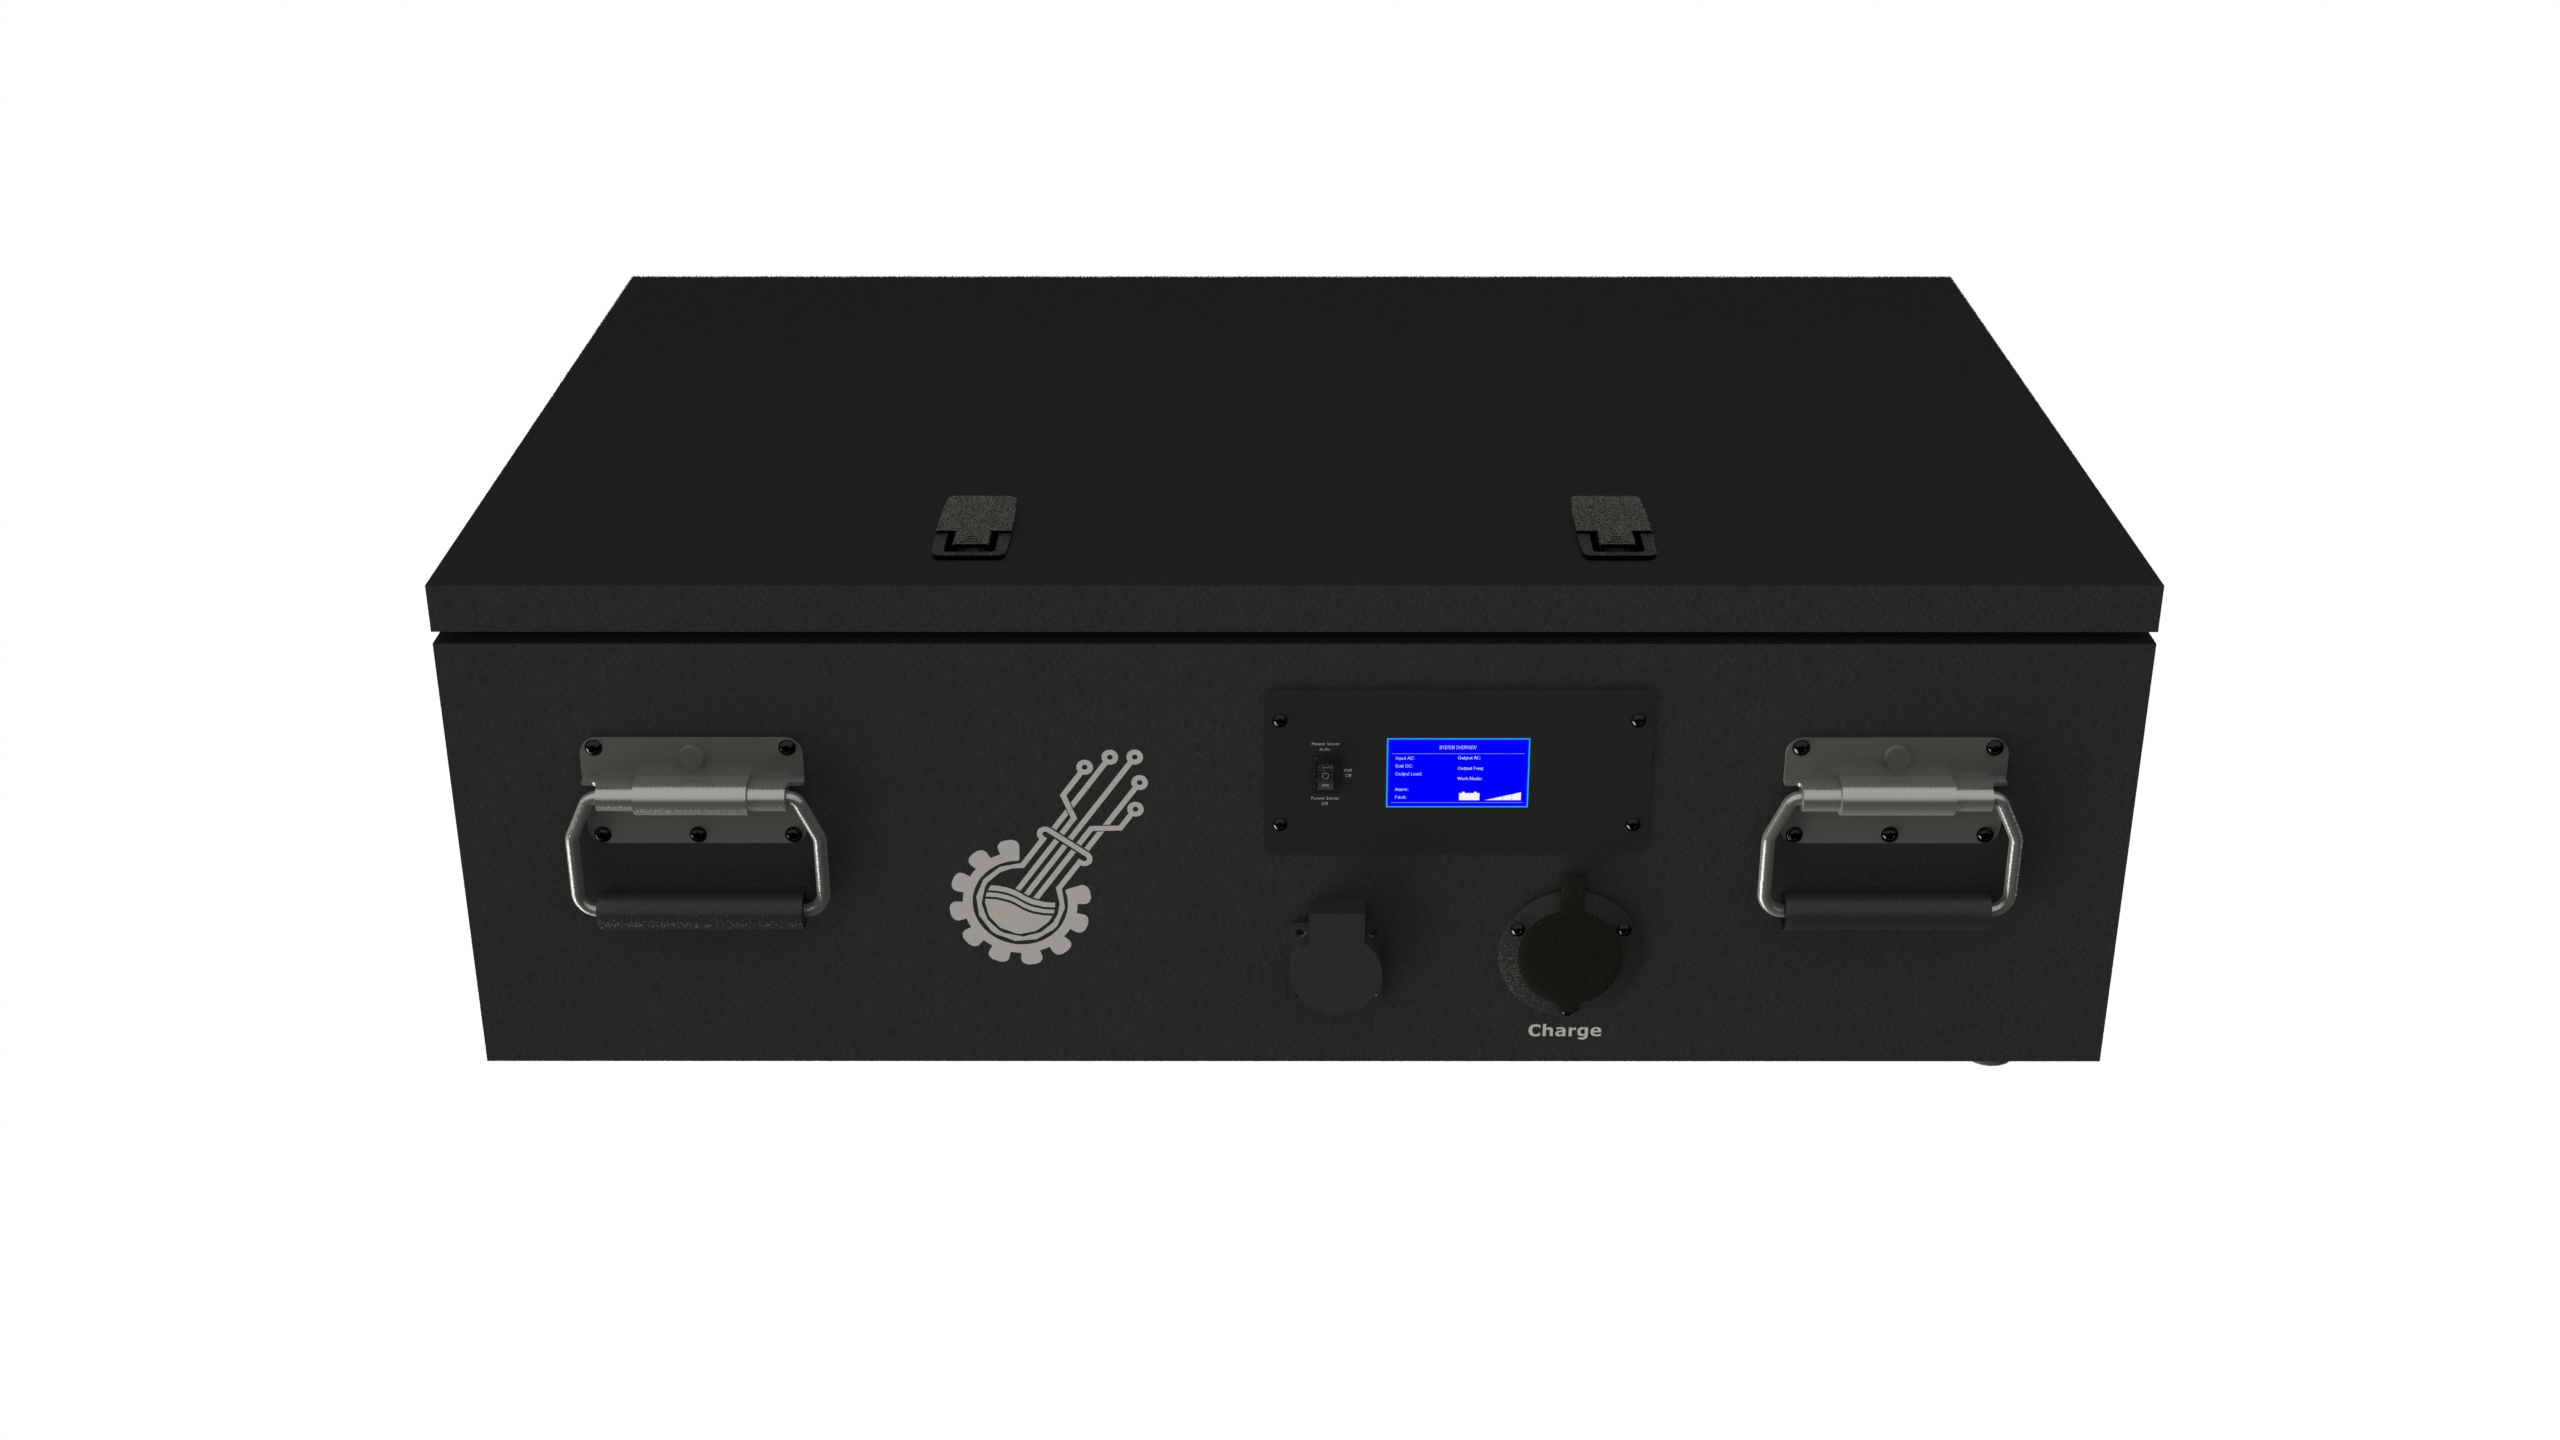
\includegraphics[width=6in]{top_front_closed.jpg}

\end{flushleft}
\end{document}